\chapter{Fermiones, matrices de Dirac y mar de Dirac}

El mar de Dirac es nuestro destino, pero la ruta importa. Antes de abordar la energía negativa en la teoría relativista del electrón, necesitamos dos herramientas. Primero, el álgebra de operadores que distingue los fermiones de los bosones. Después, repasaremos la ecuación de Dirac unidimensional, donde cada ampliación de la función de onda puede verse sin la geometría de tres dimensiones espaciales. Con esas piezas ya dispuestas, la ecuación tridimensional impondrá su propia estructura matricial, y la discusión inicial de los estados fermiónicos ocupados y vacíos volverá a ser la clave para entender los positrones.

Usamos \(c=\hbar=1\). La letra mayúscula \(P\) denota un operador de momento; la minúscula \(p\), un autovalor del momento; y los símbolos en negrita, sus versiones tridimensionales.

\section{El intercambio se convierte en álgebra de operadores}

Consideremos dos partículas idénticas, una en \(x\) y otra en \(y\). Las etiquetas \(x\) y \(y\) denotan posiciones completas; no son dos coordenadas cartesianas de una sola partícula. Al actuar sobre el vacío con dos operadores de creación se obtiene
\begin{equation}
\lvert x,y\rangle
=
\psi^\dagger(x)\psi^\dagger(y)\lvert0\rangle.
\label{eq:l10-two-particle-state}
\end{equation}

Para los bosones, intercambiar las dos posiciones deja el estado inalterado:
\begin{equation}
\lvert x,y\rangle=\lvert y,x\rangle.
\end{equation}
La afirmación sobre los operadores que garantiza esta simetría es
\begin{equation}
\psi^\dagger(x)\psi^\dagger(y)
=
\psi^\dagger(y)\psi^\dagger(x).
\label{eq:l10-boson-exchange}
\end{equation}
Dos operadores de creación bosónicos conmutan, así que podemos invertir su orden sin cambiar el estado que crean.

Para los fermiones, el intercambio cambia el signo:
\begin{equation}
\lvert x,y\rangle=-\lvert y,x\rangle.
\label{eq:l10-fermion-state-exchange}
\end{equation}
El signo global de un vector de estado aislado no es observable, pero sí lo son los signos relativos entre alternativas, así que hay que conservar este signo menos de manera consistente. La ecuación~\eqref{eq:l10-fermion-state-exchange} exige
\begin{equation}
\psi^\dagger(x)\psi^\dagger(y)
=
-\,\psi^\dagger(y)\psi^\dagger(x).
\label{eq:l10-fermion-operator-exchange}
\end{equation}

\begin{figure}[htbp]
\centering
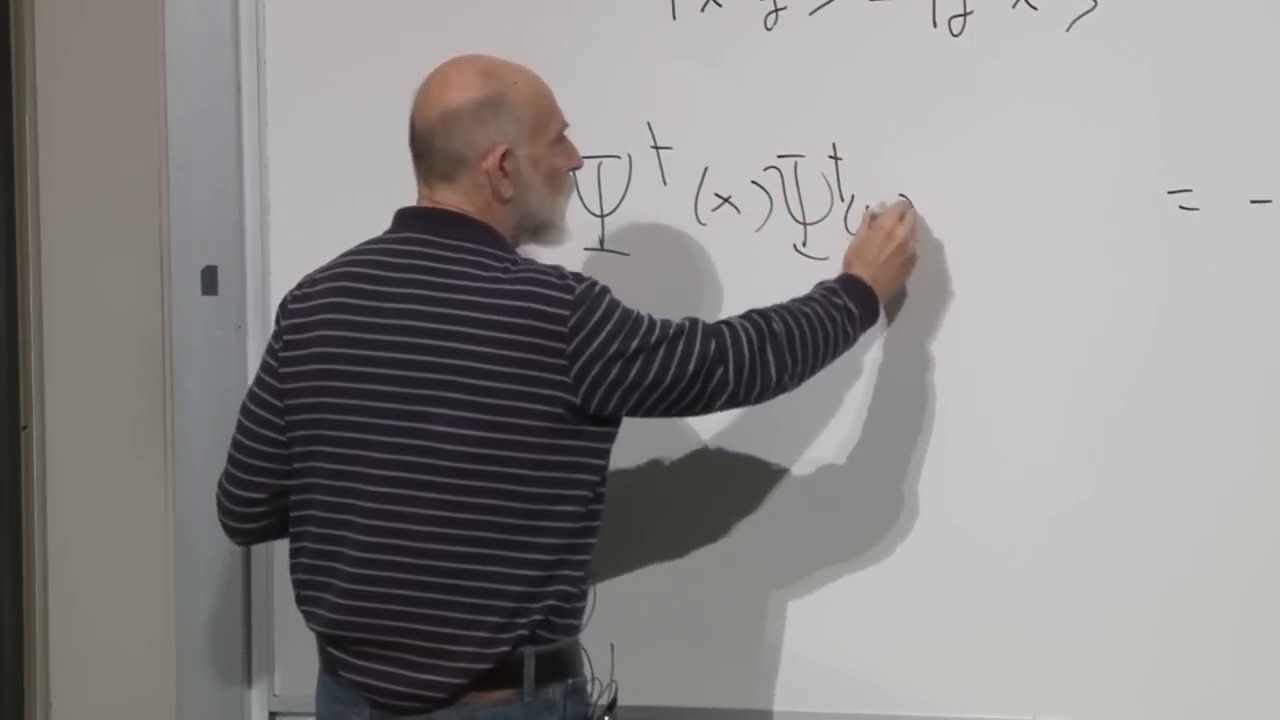
\includegraphics[width=0.94\linewidth]{lecture_10_figure_02.png}
\caption{La relación en la pizarra que implementa el intercambio fermiónico. Al intercambiar los operadores de creación, cambia el signo del estado de dos partículas.}
\lectureframe{00:05:50}
\end{figure}

Para dos operadores cualesquiera \(A\) y \(B\), definimos el anticonmutador como
\begin{equation}
\{A,B\}:=AB+BA.
\end{equation}
Por tanto, la regla de intercambio es
\begin{equation}
\{\psi^\dagger(x),\psi^\dagger(y)\}=0.
\label{eq:l10-creation-anticommutator}
\end{equation}
El álgebra correspondiente de los campos fermiónicos sustituye los conmutadores bosónicos por anticonmutadores. Hay que distinguir los dos usos de la palabra: los operadores de campo anticonmutan debido a la estadística de Fermi, mientras que más adelante las matrices anticonmutarán para cancelar términos cruzados en una relación de dispersión relativista.

Ahora tomemos \(y=x\) en la ecuación~\eqref{eq:l10-creation-anticommutator}. Ambos productos pasan a ser iguales:
\begin{align}
0
&=\{\psi^\dagger(x),\psi^\dagger(x)\}\\
&=2\,\psi^\dagger(x)\psi^\dagger(x).
\end{align}
Por tanto,
\begin{equation}
\bigl(\psi^\dagger(x)\bigr)^2=0.
\label{eq:l10-exclusion}
\end{equation}
Intentar crear dos fermiones idénticos en el mismo estado de una partícula da el vector nulo. Esta es la expresión en términos de operadores del principio de exclusión.

\begin{figure}[htbp]
\centering
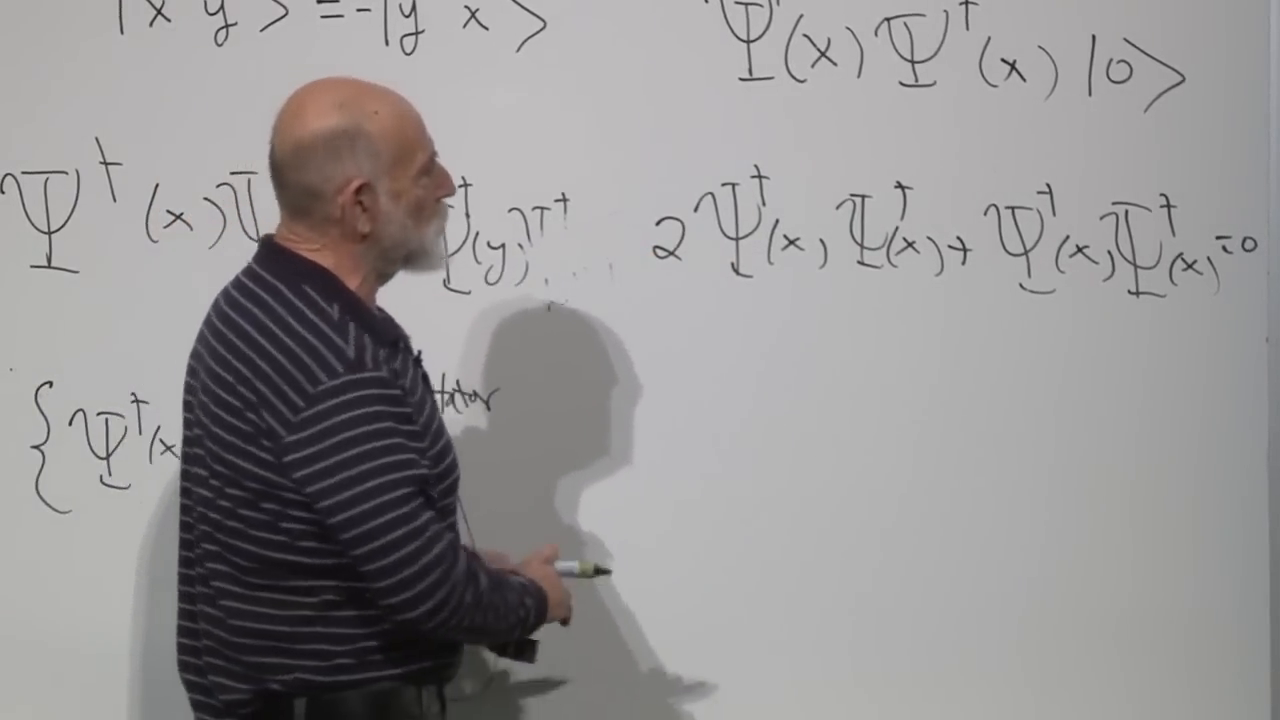
\includegraphics[width=0.94\linewidth]{lecture_10_figure_03.png}
\caption{El caso particular de estados iguales en la pizarra. El producto repetido de operadores de creación aparece dos veces y, por tanto, debe anularse.}
\lectureframe{00:08:04}
\end{figure}

\begin{figure}[htbp]
\centering
\begin{adjustbox}{max width=\linewidth}
\begin{tikzpicture}[node distance=1.25cm,>=Latex]
\node[draw,rounded corners,align=center,inner sep=7pt] (a)
  {$\{\psi^\dagger(x),\psi^\dagger(x)\}=0$};
\node[draw,rounded corners,align=center,inner sep=7pt,right=of a] (b)
  {$2(\psi^\dagger(x))^2=0$};
\node[draw,rounded corners,align=center,inner sep=7pt,right=of b] (c)
  {$(\psi^\dagger(x))^2=0$};
\draw[->,thick] (a) -- (b);
\draw[->,thick] (b) -- (c);
\end{tikzpicture}
\end{adjustbox}
\caption{La demostración de la exclusión, reconstruida sin el trabajo intermedio parcialmente borrado de la pizarra.}
\end{figure}

\section{Por qué para un fermión los estados ocupado y vacío son simétricos}

Hay una segunda diferencia entre los operadores bosónicos y fermiónicos, más sutil que la exclusión y esencial más adelante. Para un modo bosónico,
\begin{equation}
[a,a^\dagger]=1,
\qquad
n=0,1,2,\ldots.
\end{equation}
Intercambiar \(a\) y \(a^\dagger\) cambia el signo del conmutador. Aunque a los operadores se los llamara simplemente \(A\) y \(B\), el álgebra nos diría cuál de los órdenes aumenta el número de ocupación y cuál lo disminuye.

La escalera de ocupación bosónica también tiene una orientación. El operador de aniquilación acaba por llegar a \(\lvert0\rangle\) y da cero, mientras que el operador de creación puede continuar indefinidamente:
\begin{align}
a\lvert0\rangle&=0,\\
a^\dagger\lvert n\rangle&\propto\lvert n+1\rangle,
\qquad n=0,1,2,\ldots.
\end{align}
Invertir esta escalera no reproduce el mismo espectro. Hay un extremo inferior, pero no uno superior.

Para un modo fermiónico,
\begin{equation}
\{a,a^\dagger\}=1,
\qquad
a^2=(a^\dagger)^2=0,
\qquad
n=0,1.
\label{eq:l10-fermion-mode}
\end{equation}
El operador de creación lleva el estado vacío al estado ocupado y luego se detiene:
\begin{equation}
a^\dagger\lvert0\rangle=\lvert1\rangle,
\qquad
a^\dagger\lvert1\rangle=0.
\end{equation}
El operador de aniquilación hace lo contrario:
\begin{equation}
a\lvert1\rangle=\lvert0\rangle,
\qquad
a\lvert0\rangle=0.
\end{equation}
Solo hay dos estados, así que el diagrama es simétrico al intercambiar ocupado por vacío y \(a\) por \(a^\dagger\). Los operadores siguen teniendo significados físicos distintos, pero su álgebra ya no destaca uno como operador de creación y al otro como operador de aniquilación. Esta simetría formal es el germen de la reinterpretación en términos de partículas y huecos.

\begin{classroomqa}
\lecturetimestamp{00:13:54}
\audiencequestion{Si \((a^\dagger)^2=0\), ¿es una contradicción o implica que \(a^\dagger=0\)?}
\lecturerresponse{Ninguna de las dos cosas. Un operador no nulo puede tener cuadrado nulo. Aquí, \(a^\dagger\) lleva \(\lvert0\rangle\) a \(\lvert1\rangle\), pero no hay ningún estado permitido por encima de \(\lvert1\rangle\), así que aplicarlo dos veces da cero. El mismo razonamiento da \(a^2=0\).}
\end{classroomqa}

Tengamos presente esta simetría entre ocupado y vacío. Cuando se elimine un electrón de energía negativa, el operador de aniquilación se reinterpretará como operador de creación de positrones. No es un cambio arbitrario de notación: se apoya exactamente en el álgebra fermiónica de dos estados establecida aquí.

\section{La construcción de Dirac en una dimensión}

Volvamos ahora a una partícula en una dimensión espacial. La ecuación de onda relativista de primer orden más sencilla es
\begin{equation}
i\partial_t\psi=-\,i\partial_x\psi.
\label{eq:l10-right-mover}
\end{equation}
Con \(P=-i\partial_x\), queda
\begin{equation}
H=P.
\end{equation}
Un estado propio del momento tiene \(E=p\), y su velocidad de grupo es
\begin{equation}
v_g=\frac{dE}{dp}=1.
\end{equation}
Tanto el momento positivo como el negativo y, por tanto, tanto la energía positiva como la negativa dan lugar a una onda que se propaga rígidamente hacia la derecha. El signo de \(p\) cambia el patrón de fase, no el sentido de propagación.

Una partícula con masa debe poder moverse en cualquiera de los dos sentidos. Introduzcamos una segunda componente que satisfaga
\begin{equation}
H\psi_1=P\psi_1,
\qquad
H\psi_2=-P\psi_2.
\label{eq:l10-two-directions}
\end{equation}
La primera componente se propaga hacia la derecha; la segunda, hacia la izquierda. Reunámoslas en una columna,
\begin{equation}
\Psi=
\begin{pmatrix}
\psi_1\\
\psi_2
\end{pmatrix},
\end{equation}
y definamos
\begin{equation}
\alpha=
\begin{pmatrix}
1&0\\
0&-1
\end{pmatrix}.
\end{equation}
Ambas ecuaciones pasan a ser
\begin{equation}
H\Psi=\alpha P\Psi.
\label{eq:l10-massless-one-d}
\end{equation}
Incluir los dos sentidos tiene como coste un nuevo grado de libertad interno con dos valores.

La dirección por sí sola no produce la masa. Introduzcamos una segunda matriz,
\begin{equation}
\beta=
\begin{pmatrix}
0&1\\
1&0
\end{pmatrix},
\end{equation}
y probemos
\begin{equation}
H=\alpha P+\beta m.
\label{eq:l10-massive-one-d}
\end{equation}
Las matrices satisfacen
\begin{equation}
\alpha^2=\beta^2=\mathbb{1},
\qquad
\{\alpha,\beta\}=0.
\label{eq:l10-one-d-algebra}
\end{equation}
Al elevar el hamiltoniano al cuadrado se obtiene
\begin{align}
H^2
&=(\alpha P+\beta m)^2\\
&=\alpha^2P^2+\beta^2m^2
  +(\alpha\beta+\beta\alpha)Pm\\
&=P^2+m^2.
\label{eq:l10-one-d-dispersion}
\end{align}
El anticonmutador de la ecuación~\eqref{eq:l10-one-d-algebra} elimina el término no deseado que es lineal tanto en \(P\) como en \(m\).

La matriz no diagonal \(\beta\) acopla las dos componentes de dirección. Conviene imaginar el término de masa como una mezcla continua de las amplitudes que se propagan hacia la derecha y hacia la izquierda. No hay que tomar literalmente esta imagen como una partícula que rebota de un lado a otro por una trayectoria microscópica, pero sí ayuda a entender por qué un paquete de ondas masivo puede tener una velocidad media menor que la de la luz y un sistema de reposo, mientras que una componente quiral sin masa aislada no puede.

\begin{classroomqa}
\lecturetimestamp{00:23:37}
\audiencequestion{¿Hay una interpretación física más profunda de introducir ambas componentes de dirección?}
\lecturerresponse{Sí, pero se aprecia con más claridad en tres dimensiones. En esta etapa, son simplemente las dos componentes necesarias para describir propagaciones en sentidos opuestos y admitir un acoplamiento de masa no diagonal. Más adelante se interpretarán en términos de quiralidad, o helicidad.}
\end{classroomqa}

\section{Tres dimensiones exigen las matrices de Pauli}

En tres dimensiones espaciales, el momento es un vector. Un hamiltoniano lineal en el momento y escalar bajo rotaciones sugiere, por tanto, otro vector, esta vez un vector cuyas componentes son matrices:
\begin{equation}
H=\boldsymbol{\alpha}\cdot\mathbf P
=\alpha_xP_x+\alpha_yP_y+\alpha_zP_z.
\label{eq:l10-three-d-ansatz}
\end{equation}

\begin{figure}[htbp]
\centering
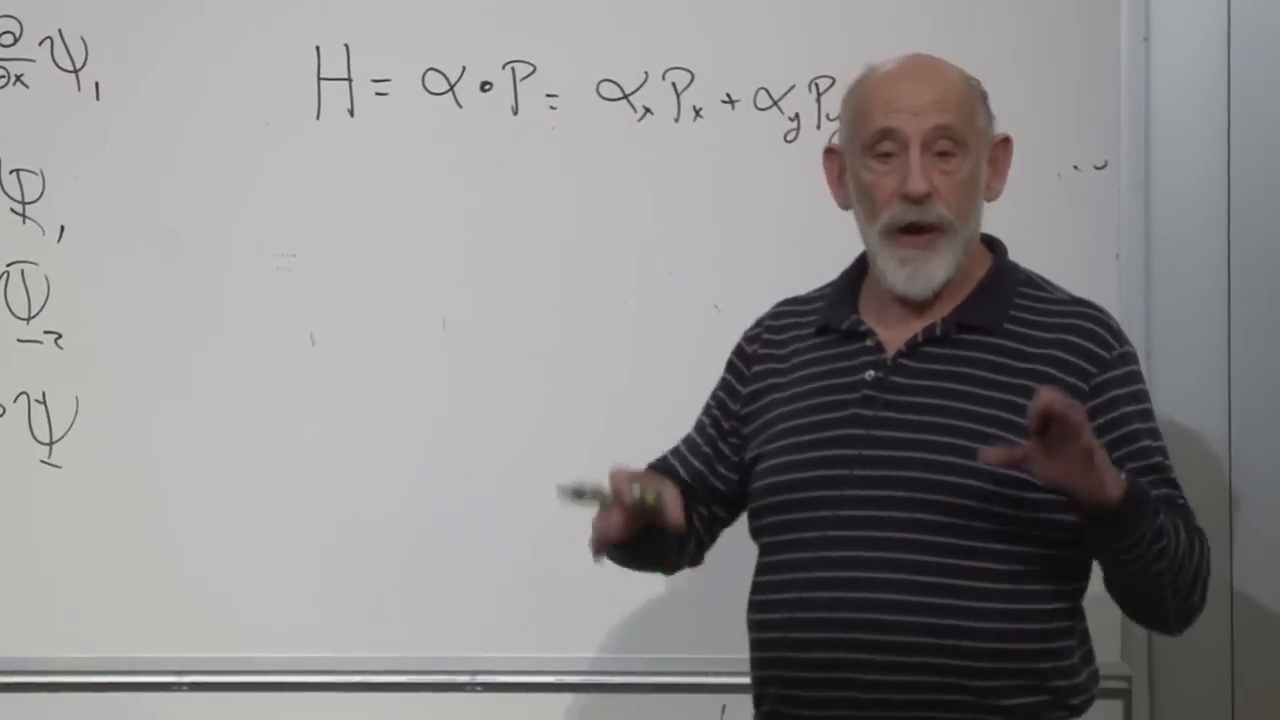
\includegraphics[width=0.94\linewidth]{lecture_10_figure_04.png}
\caption{El ansatz sin masa tridimensional \(H=\boldsymbol{\alpha}\cdot\mathbf P\) en el punto en que una matriz pasa a ser un vector de tres matrices.}
\lectureframe{00:26:00}
\end{figure}

Empecemos de nuevo con el caso sin masa. Exigimos
\begin{equation}
H^2=\mathbf P^2=P_x^2+P_y^2+P_z^2.
\end{equation}
Al desarrollar el cuadrado de la ecuación~\eqref{eq:l10-three-d-ansatz},
\begin{align}
H^2
&=\alpha_x^2P_x^2+\alpha_y^2P_y^2\\
&\quad+\alpha_z^2P_z^2\\
&\quad+\{\alpha_x,\alpha_y\}P_xP_y\\
&\quad+\{\alpha_x,\alpha_z\}P_xP_z\\
&\quad+\{\alpha_y,\alpha_z\}P_yP_z.
\end{align}
Los términos diagonales son los correctos si
\begin{equation}
\alpha_x^2=\alpha_y^2=\alpha_z^2=\mathbb{1},
\end{equation}
y todos los términos cruzados desaparecen si
\begin{equation}
\{\alpha_i,\alpha_j\}=0,
\qquad i\ne j.
\label{eq:l10-alpha-anticommutation}
\end{equation}

Tres matrices familiares \(2\times2\) hacen exactamente esto:
\begin{equation}
\sigma_x=
\begin{pmatrix}
0&1\\
1&0
\end{pmatrix},
\quad
\sigma_y=
\begin{pmatrix}
0&-i\\
i&0
\end{pmatrix},
\quad
\sigma_z=
\begin{pmatrix}
1&0\\
0&-1
\end{pmatrix}.
\label{eq:l10-pauli-matrices}
\end{equation}
Así, una solución es
\begin{equation}
\alpha_i=\sigma_i,
\qquad
H=\boldsymbol{\sigma}\cdot\mathbf P.
\label{eq:l10-weyl-hamiltonian}
\end{equation}

\begin{figure}[htbp]
\centering
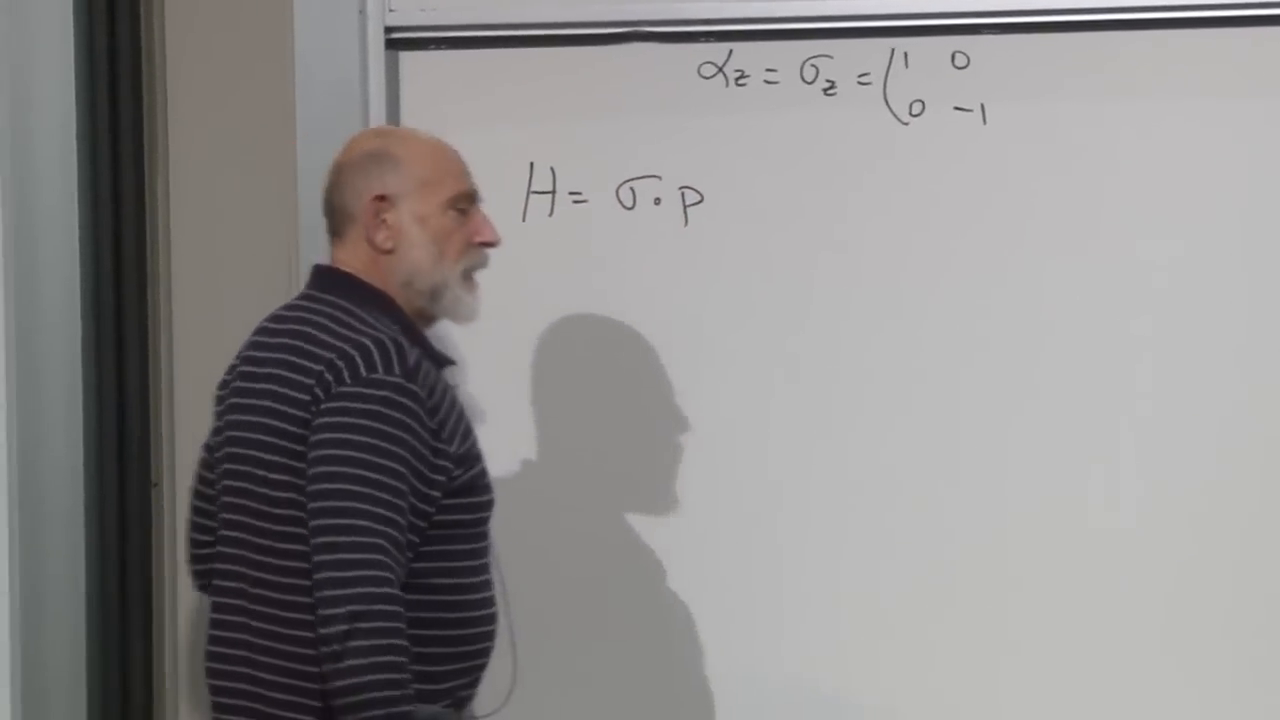
\includegraphics[width=0.94\linewidth]{lecture_10_figure_05.png}
\caption{El hamiltoniano sin masa en su forma compacta \(H=\boldsymbol{\sigma}\cdot\mathbf P\), con \(\alpha_z=\sigma_z\) aún visible encima.}
\lectureframe{00:28:16}
\end{figure}

Para un estado propio del momento,
\begin{equation}
\boldsymbol{\sigma}\cdot\mathbf p
=
|\mathbf p|\,\boldsymbol{\sigma}\cdot\widehat{\mathbf p}.
\end{equation}
El operador \(\boldsymbol{\sigma}\cdot\widehat{\mathbf p}\) tiene autovalores \(+1\) y \(-1\), así que
\begin{equation}
E=\pm|\mathbf p|.
\end{equation}
En esta teoría de dos componentes, para la energía positiva el grado de libertad de Pauli está alineado con el momento; para la energía negativa, está antialineado. La alineación está fijada: no es una dirección de espín que pueda ajustarse independientemente para un signo de energía dado.

\begin{classroomqa}
\lecturetimestamp{00:30:10}
\audiencequestion{¿El espín surge como consecuencia de la ecuación de Dirac o se introdujo porque ya se sabía que el electrón tiene momento magnético?}
\lecturerresponse{Aquí, «surgir» significa «aparecer como consecuencia», no «desaparecer». El punto de partida fue exigir un hamiltoniano lineal en el momento cuyo cuadrado fuera \(\mathbf P^2\). Los números ordinarios no pueden satisfacer el álgebra requerida, pero las matrices de Pauli sí. Por tanto, su estructura de dos componentes aparece con la propia linealización. Esto no demuestra que todas las partículas deban tener espín; indica que las partículas descritas por esta ecuación de tipo Dirac tienen el grado de libertad espinorial correspondiente.}
\end{classroomqa}

Esta es una de las lecciones centrales de la construcción. Las matrices no son etiquetas decorativas que se añaden después de encontrar la ecuación relativista. Surgen al intentar obtener una raíz cuadrada local de la relación de dispersión relativista.

\section{Por qué la masa requiere cuatro componentes}

Intentemos repetir la construcción unidimensional de la masa sin ampliar la teoría \(2\times2\):
\begin{equation}
H=\boldsymbol{\sigma}\cdot\mathbf P+\beta m.
\label{eq:l10-failed-mass}
\end{equation}
Supongamos que \(\beta^2=\mathbb{1}\). El cuadrado contiene los términos deseados \(\mathbf P^2+m^2\), pero también contiene
\begin{equation}
m\sum_i\{\sigma_i,\beta\}P_i.
\end{equation}
Para eliminar este término, una matriz \(\beta\) tendría que satisfacer
\begin{equation}
\{\sigma_x,\beta\}
=
\{\sigma_y,\beta\}
=
\{\sigma_z,\beta\}
=0.
\label{eq:l10-impossible-beta}
\end{equation}
Ninguna matriz \(2\times2\) lo hace. La identidad conmuta con las tres matrices de Pauli, y toda matriz \(2\times2\) sin traza es una combinación lineal de matrices de Pauli. Cualquier combinación así deja de anticonmutar con la componente paralela a ella. El álgebra \(2\times2\) no contiene una cuarta matriz independiente del tipo requerido.

La solución consiste en ampliar el espinor. Cuatro matrices que anticonmutan entre sí y cuyo cuadrado es la identidad aparecen por primera vez en una representación compleja \(4\times4\). Este tamaño matricial no se elige porque el espacio-tiempo tenga cuatro dimensiones; es el espacio matricial más pequeño capaz de realizar el álgebra requerida.

Hay muchas representaciones equivalentes. Un cambio unitario de base del espinor modifica las entradas de todas las matrices sin cambiar ninguna predicción física. Lo que importa es el conjunto abstracto de relaciones
\begin{equation}
\{\alpha_i,\alpha_j\}=2\delta_{ij}\mathbb{1},
\qquad
\{\alpha_i,\beta\}=0,
\qquad
\beta^2=\mathbb{1}.
\label{eq:l10-dirac-algebra}
\end{equation}

\begin{classroomqa}
\lecturetimestamp{00:37:38}
\audiencequestion{¿Puede considerarse \(\beta\) una componente temporal \(\alpha_t\)?}
\lecturerresponse{No directamente. Las tres \(\alpha_i\) no se combinan con \(\beta\) como las cuatro componentes de un solo vector de Lorentz. En notación covariante se definen, en cambio, \(\beta=\gamma^0\) y \(\alpha_i=\gamma^0\gamma^i\); las cuatro matrices \(\gamma^\mu\) satisfacen el álgebra de Clifford del espacio-tiempo.}
\end{classroomqa}

Una representación por bloques conveniente es
\begin{equation}
\alpha_i=
\begin{pmatrix}
\sigma_i&0\\
0&-\sigma_i
\end{pmatrix},
\qquad
\beta=
\begin{pmatrix}
0&I_2\\
I_2&0
\end{pmatrix}.
\label{eq:l10-block-representation}
\end{equation}
Las matrices de Pauli en los bloques diagonales garantizan que distintas \(\alpha_i\) anticonmuten. Los bloques de identidad no diagonales de \(\beta\) garantizan que \(\beta\) anticonmute con cada \(\alpha_i\).

\begin{figure}[htbp]
\centering
\includegraphics[width=0.94\linewidth]{lecture_10_figure_06.png}
\caption{La representación por bloques \(4\times4\) de la pizarra. Las ecuaciones superiores recogen los anticonmutadores requeridos; las matrices completas aparecen compuestas en la ecuación~\eqref{eq:l10-block-representation}.}
\lectureframe{00:41:10}
\end{figure}

Ahora el hamiltoniano con masa es
\begin{equation}
H=\boldsymbol{\alpha}\cdot\mathbf P+\beta m
=
\begin{pmatrix}
\boldsymbol{\sigma}\cdot\mathbf P&mI_2\\
mI_2&-\boldsymbol{\sigma}\cdot\mathbf P
\end{pmatrix}.
\label{eq:l10-massive-dirac}
\end{equation}
Usando la ecuación~\eqref{eq:l10-dirac-algebra},
\begin{equation}
H^2=\mathbf P^2+m^2.
\end{equation}
Por tanto, la estructura de cuatro componentes no es un añadido opcional. Es la estructura más pequeña que permite incluir tanto el momento tridimensional como un término de masa y mantener la ecuación de primer orden.

\section{La quiralidad y el significado de las componentes adicionales}

¿Qué distinción física aportó la ampliación? Empecemos con el bloque superior sin masa,
\begin{equation}
H_R=\boldsymbol{\sigma}\cdot\mathbf P,
\end{equation}
y el bloque inferior sin masa,
\begin{equation}
H_L=-\boldsymbol{\sigma}\cdot\mathbf P.
\end{equation}
En los estados de energía positiva, en el primero el espín está alineado con el momento y en el segundo está antialineado. Son helicidades opuestas. En una teoría sin masa, la helicidad es invariante bajo transformaciones de Lorentz propias, porque ningún observador puede sobrepasar a una partícula de tipo luz e invertir su momento sin dejar inalterado su espín. Por tanto, los dos bloques describen sectores quirales opuestos.

\begin{classroomqa}
\lecturetimestamp{00:41:28}
\audiencequestion{En una dimensión se necesitaba un grado de libertad binario adicional para introducir la masa. ¿Cuál es la distinción física correspondiente en tres dimensiones?}
\lecturerresponse{Es la quiralidad del espinor. Los dos bloques \(2\times2\) describen relaciones opuestas entre el espín y el momento. Uno es dextrógiro y el otro levógiro. La teoría \(4\times4\) contiene ambos.}
\end{classroomqa}

El término de masa en la ecuación~\eqref{eq:l10-massive-dirac} es no diagonal. Lleva una amplitud del bloque superior al inferior y viceversa:
\begin{equation}
\beta m
\begin{pmatrix}
\Psi_R\\
\Psi_L
\end{pmatrix}
=
m
\begin{pmatrix}
\Psi_L\\
\Psi_R
\end{pmatrix}.
\end{equation}
Por tanto, la masa acopla quiralidades opuestas.

\begin{classroomqa}
\lecturetimestamp{00:43:58}
\audiencequestion{¿Puede una partícula sin masa cambiar de quiralidad?}
\lecturerresponse{No en el hamiltoniano libre sin masa que se muestra aquí. Los dos bloques están desacoplados, así que un estado que comienza con quiralidad dextrógira o levógira la conserva. El término de masa no diagonal es precisamente lo que los mezcla cuando \(m\ne0\).}
\end{classroomqa}

Este lenguaje es exacto para la representación por bloques, pero no hay que llevar demasiado lejos la imagen de una partícula que alterna mecánicamente entre dos flechas. La afirmación física es el acoplamiento matricial en la ecuación de onda.

\begin{classroomqa}
\lecturetimestamp{00:44:50}
\audiencequestion{¿Están estas matrices incorporadas en los cuaterniones?}
\lecturerresponse{Las matrices de Pauli están estrechamente relacionadas con las unidades cuaterniónicas: las matrices \(-i\sigma_i\) al cuadrado dan \(-\mathbb{1}\) y se multiplican siguiendo el patrón cuaterniónico, salvo por las convenciones de orientación. Las matrices de Dirac completas requieren el álgebra de Clifford, más amplia, y la conexión con los cuaterniones no es necesaria para el argumento que sigue.}
\end{classroomqa}

\begin{classroomqa}
\lecturetimestamp{00:46:34}
\audiencequestion{Si el espín es momento angular, ¿hay aquí un término de energía independiente asociado a él?}
\lecturerresponse{No se añade ningún término independiente para la partícula libre. La estructura espinorial ya aparece en el hamiltoniano cinético a través de las matrices. Acoplar el espín a un campo magnético externo introduciría términos de interacción adicionales, pero ese es otro problema.}
\end{classroomqa}

\section{Las matrices alfa representan la velocidad, no el espín}

Cada \(\alpha_i\) tiene dos autovalores iguales a \(+1\) y dos iguales a \(-1\). Las distintas componentes no conmutan, así que no se pueden medir todas simultáneamente con precisión. Para identificar qué representa una de ellas, usemos la ecuación de Heisenberg. Para un operador \(L\) sin dependencia explícita del tiempo,
\begin{equation}
\dot L=i[H,L].
\label{eq:l10-heisenberg}
\end{equation}
La convención de signos queda fijada aquí por la evolución de Schr\"odinger \(e^{-iHt}\).

Apliquemos la ecuación~\eqref{eq:l10-heisenberg} al operador de posición \(x\). Las matrices actúan sobre los índices del espinor y conmutan con la posición, mientras que solo \(P_x\) no conmuta con \(x\):
\begin{align}
\dot x
&=i[\boldsymbol{\alpha}\cdot\mathbf P+\beta m,x]\\
&=i\alpha_x[P_x,x]\\
&=\alpha_x,
\label{eq:l10-velocity}
\end{align}
porque \([P_x,x]=-i\). Así, \(\alpha_x\) es la componente \(x\) del operador de velocidad; de manera análoga,
\begin{equation}
\dot{\mathbf x}=\boldsymbol{\alpha}.
\end{equation}

\begin{classroomqa}
\lecturetimestamp{00:51:50}
\audiencequestion{¿Una medición de una componente de la velocidad da realmente solo \(+1\) o \(-1\)?}
\lecturerresponse{Sí, para el operador instantáneo \(\alpha_i\) en unidades en las que \(c=1\). Un estado general no tiene por qué ser un estado propio, así que su valor esperado puede estar en cualquier punto entre esos valores. El paquete de ondas que se transporta suavemente tiene una velocidad media inferior a la de la luz cuando la partícula tiene masa.}
\end{classroomqa}

La velocidad no se conserva:
\begin{equation}
\dot\alpha_x=i[H,\alpha_x]\ne0.
\end{equation}
Los términos que contienen \(\alpha_y\), \(\alpha_z\) y \(\beta\) no conmutan con \(\alpha_x\). Por consiguiente, un estado que contenga componentes de energía tanto positiva como negativa presenta una contribución oscilatoria rápida a su posición. Esto es el \emph{zitterbewegung}, literalmente, movimiento tembloroso.

Tras promediar en tiempos largos comparados con la rápida oscilación, la velocidad relativista esperada es
\begin{equation}
\overline{\mathbf v}=\frac{\mathbf p}{E},
\end{equation}
que para un electrón lento se reduce a \(\mathbf p/m\).

\begin{classroomqa}
\lecturetimestamp{00:54:40}
\audiencequestion{¿Que un electrón libre tiemble sin fuerza externa contradice la ley de Newton?}
\lecturerresponse{No. La invariancia traslacional conserva el momento, de modo que \(\dot{\mathbf P}=0\). El operador de velocidad de Dirac no es simplemente \(\mathbf P/m\), y su parte rápidamente oscilatoria puede cambiar aunque el momento permanezca fijo. El movimiento promediado en el tiempo obedece la relación esperada para una partícula libre.}
\end{classroomqa}

\begin{classroomqa}
\lecturetimestamp{00:55:22}
\audiencequestion{¿La velocidad es siempre \(c\)?}
\lecturerresponse{Una medición instantánea de una componente \(\alpha_i\) tiene autovalores \(\pm c\), pero un paquete de ondas masivo es, en general, una superposición y tiene un valor esperado sublumínico. Su velocidad de grupo media es \(\mathbf p/E\).}
\end{classroomqa}

\begin{classroomqa}
\lecturetimestamp{00:55:30}
\audiencequestion{¿Se puede imaginar la oscilación como si la masa hiciera variar la velocidad?}
\lecturerresponse{No. La masa es un parámetro fijo. La oscilación se debe a que los operadores de velocidad y de hamiltoniano no conmutan o, equivalentemente, a la interferencia entre sectores de energía; no se debe a una masa fluctuante.}
\end{classroomqa}

\begin{classroomqa}
\lecturetimestamp{00:56:22}
\audiencequestion{¿Podría una medición instantánea encontrar la velocidad apuntando en un sentido aunque el movimiento medio apunte en otro?}
\lecturerresponse{Sí. El operador de la componente tiene los dos autovalores definidos, mientras que las mediciones repetidas o promediadas en el tiempo recuperan la deriva más suave.}
\end{classroomqa}

También hay que usar con cuidado la palabra espín. Las \(\alpha_i\) se transforman como componentes de la velocidad, que es un vector ordinario. El operador de espín propiamente dicho en esta representación es
\begin{equation}
\mathbf S=\frac12\boldsymbol{\Sigma},
\qquad
\Sigma_i=
\begin{pmatrix}
\sigma_i&0\\
0&\sigma_i
\end{pmatrix}.
\label{eq:l10-spin-operator}
\end{equation}
Difiere de \(\alpha_i\) en el signo del bloque inferior. Las matrices están estrechamente relacionadas, pero la velocidad y el espín no son el mismo observable.

\section{La energía negativa y el vacío de energía mínima}

El problema de la energía negativa ya estaba presente antes de introducir toda esta maquinaria matricial. Volvamos al modo que se propaga hacia la derecha en una dimensión,
\begin{equation}
H=P.
\end{equation}
Como \(p\) recorre toda la recta real, \(E=p\) no está acotada inferiormente.

El vacío no puede significar simplemente un estado sin partículas. Debe ser el estado al que ya no se le pueda extraer energía. Si un estado vacío permite añadir una partícula de energía negativa, reducir la energía, añadir otra y continuar indefinidamente, entonces ese estado no es un vacío estable.

La estadística de Fermi ofrece una salida histórica. Coloquemos un electrón en cada estado de energía negativa. Cada electrón añadido reduce la energía total, pero la exclusión permite un solo electrón en cada estado de una partícula. Una vez ocupados todos los estados de energía negativa, ningún electrón adicional puede caer en ese sector. Dirac identificó esta configuración llena como el vacío.

La misma construcción no funcionaría para los bosones. Se pueden ocupar con un número arbitrario de bosones un mismo estado, así que un modo bosónico de energía negativa podría absorber partículas sin límite. El límite fermiónico \(n=0,1\), introducido al comienzo de la clase, es precisamente lo que detiene el descenso.

\begin{figure}[htbp]
\centering
\includegraphics[width=0.94\linewidth]{lecture_10_figure_07.png}
\caption{La imagen histórica del mar de Dirac en la pizarra: una escalera de niveles de energía negativa llenos hasta la línea divisoria, con estados de energía positiva por encima.}
\lectureframe{01:02:45}
\end{figure}

\begin{figure}[htbp]
\centering
\begin{adjustbox}{max width=\linewidth}
\begin{tikzpicture}[x=1.05cm,y=0.72cm,>=Latex]
\draw[->] (0,-4.8) -- (0,4.8) node[above] {$E$};
\draw[thick] (-2.9,0) -- (3.2,0) node[right] {$E=0$};
\foreach \y in {-4,-3.3,...,-0.5} {
  \draw (-2.3,\y) -- (2.3,\y);
  \foreach \x in {-1.8,-1.2,...,1.8} {
    \fill[blue!65!black] (\x,\y) circle (1.6pt);
  }
}
\foreach \y in {0.8,1.6,...,4.0} {
  \draw (-2.3,\y) -- (2.3,\y);
}
\draw[red,very thick] (0.6,-2.6) circle (5pt);
\draw[red,->,very thick] (0.6,-2.35) .. controls (1.4,-0.4) and (1.2,1.6) .. (1.5,2.4);
\fill[red] (1.5,2.4) circle (2.5pt);
\node[right,red] at (0.85,-2.6) {hole};
\node[right,red] at (1.7,2.4) {$e^-$};
\node[left] at (-2.5,-2.2) {filled negative-energy states};
\end{tikzpicture}
\end{adjustbox}
\caption{Una reconstrucción clara de la excitación sobre un mar lleno: al promover un electrón de energía negativa queda un hueco de energía positiva.}
\end{figure}

La imagen del mar es una forma histórica de expresar una reordenación correcta de los operadores. No hay que confundir su carga y energía infinitas literales con magnitudes directamente observables; la reformulación moderna elimina la necesidad de imaginar electrones materiales que llenan el espacio.

\section{Un hueco es un positrón}

Con todos los estados de energía negativa ocupados, hay dos tipos posibles de excitación. Podemos añadir un electrón de energía positiva por encima del mar, o quitar un electrón de energía negativa y dejar un hueco.

El hueco tiene la carga opuesta a la del electrón que falta. Quitar una carga \(-e\) cambia la carga en \(+e\). También tiene energía de excitación positiva. Si el electrón eliminado tenía \(E_-<0\), la energía medida con respecto al vacío lleno cambia en
\begin{equation}
E_{\mathrm{hole}}=-E_->0.
\end{equation}
El hueco es una excitación de energía positiva y carga positiva: el positrón.

Un fotón puede promover un electrón del mar a un estado de energía positiva. Con respecto al vacío, el estado final contiene un electrón y un positrón. En un diagrama ordenado en el tiempo, se suele dibujar hacia arriba el flujo del número de electrones y, para la línea del positrón, la flecha en sentido opuesto. Las flechas indican el flujo del número fermiónico o de la carga; no son pequeños vectores clásicos de velocidad.

\begin{classroomqa}
\lecturetimestamp{01:05:14}
\audiencequestion{¿Esta imagen exige que haya igual número de electrones y positrones?}
\lecturerresponse{No en un estado arbitrario. Si partimos del vacío y creamos un par neutro, obtenemos uno de cada; pero un estado puede contener ya un exceso de electrones o de positrones. La conservación de la carga restringe las reacciones, pero no exige que todos los estados permitidos tengan poblaciones iguales.}
\end{classroomqa}

Al principio, Dirac no sabía que el hueco sería una partícula de masa idéntica a la del electrón y opuesta solo en carga y otros números cuánticos aditivos. La ecuación y la construcción del hueco condujeron a esa predicción antes de que el positrón se incorporara al catálogo familiar de partículas.

\section{Un solo campo fermiónico contiene electrones y positrones}

El operador de campo incorpora la imagen histórica al álgebra moderna. Por el momento, omitamos los índices espinoriales, los factores de normalización y la dependencia temporal. Un campo unidimensional puede desarrollarse esquemáticamente como
\begin{equation}
\psi(x)
\sim
\int_{-\infty}^{\infty}dp\,a(p)e^{ipx}.
\label{eq:l10-full-field-integral}
\end{equation}
Para la relación de dispersión de propagación a la derecha \(E=p\), un valor positivo de \(p\) indica energía positiva y uno negativo de \(p\), energía negativa. Separemos la integral:
\begin{equation}
\psi(x)
\sim
\int_0^\infty dp\,a(p)e^{ipx}
+
\int_{-\infty}^0 dp\,a(p)e^{ipx}.
\end{equation}
En el segundo término, hagamos el cambio \(p=-q\), con \(q>0\), y reinterpretemos la aniquilación de un electrón de energía negativa del mar lleno como creación de un positrón:
\begin{equation}
b^\dagger(q):=a(-q).
\end{equation}
Entonces
\begin{equation}
\psi(x)
\sim
\int_0^\infty dp\,
\left[
a(p)e^{ipx}
+
b^\dagger(p)e^{-ipx}
\right].
\label{eq:l10-electron-positron-split}
\end{equation}
Los signos exactos de las fases de las ondas planas dependen de la convención de espacio-tiempo; el contenido invariante es que \(\psi\) contiene un operador de aniquilación de electrones y uno de creación de positrones.

\begin{figure}[htbp]
\centering
\includegraphics[width=0.94\linewidth]{lecture_10_figure_08.png}
\caption{La integral del campo, separada en sectores de energía positiva y negativa. En la línea inferior se reetiqueta el operador del electrón de energía negativa como operador de creación de positrones.}
\lectureframe{01:11:35}
\end{figure}

Aquí entra en juego la simetría entre ocupado y vacío de la ecuación~\eqref{eq:l10-fermion-mode}. Para los fermiones, el álgebra de operadores permite esta reinterpretación sin cambiar la estructura de anticonmutación.

Una interacción electromagnética esquemática tiene la forma
\begin{equation}
H_{\mathrm{int}}
\sim
\int dx\,\psi^\dagger(x)\psi(x)A(x),
\label{eq:l10-qed-schematic}
\end{equation}
Aquí \(A\) denota el campo del fotón. Como cada campo fermiónico contiene partes de electrón y de positrón, un solo operador local contiene varios canales:
\begin{align}
e^-&\longrightarrow e^-+\gamma,\\
e^-+e^+&\longrightarrow\gamma,\\
\gamma&\longrightarrow e^-+e^+,
\end{align}
y también sus procesos inversos y cruzados. La conservación del momento y la energía determina qué canal es cinemáticamente posible en un entorno dado. Por ejemplo, un fotón real aislado en el vacío no puede crear un par sin otro participante que absorba el retroceso, aunque el vértice local esté presente en la interacción.

\begin{figure}[htbp]
\centering
\includegraphics[width=0.94\linewidth]{lecture_10_figure_09.png}
\caption{La pizarra reúne la emisión de un electrón, la aniquilación de un par y la interacción esquemática \(\psi^\dagger\psi A\). Al seleccionar distintas partes de los mismos operadores de campo se obtienen canales distintos.}
\lectureframe{01:13:30}
\end{figure}

Así, un producto compacto de campos organiza muchas reacciones que parecen diferentes. Más adelante, Feynman formuló las reglas diagramáticas sistemáticas para calcular las amplitudes, pero buena parte de la estructura de operadores ya se ve aquí.

\section{El lenguaje moderno del vacío y la analogía del mar de Fermi}

\begin{classroomqa}
\lecturetimestamp{01:14:20}
\audiencequestion{¿Cómo describen los físicos modernos esta situación sin tratar el vacío como un mar de Dirac literal?}
\lecturerresponse{Reinterpretan directamente los operadores. Se cambia el nombre del operador de aniquilación de electrones de energía negativa por el de operador de creación de positrones de energía positiva, y se define el vacío como el estado que anulan todos los operadores de aniquilación de electrones y positrones. La formulación resultante es simétrica entre partículas y antipartículas y no requiere ningún mar material.}
\end{classroomqa}

La imagen histórica del mar sigue siendo útil porque su lógica tiene un análogo cercano en la materia condensada. En un cristal, un número fijo de electrones ocupa los estados de una partícula de menor energía disponibles hasta el nivel de Fermi. El estado fundamental lleno no está vacío. Al promover un electrón por encima de ese nivel, queda un estado desocupado por debajo. Respecto del fondo lleno, el hueco tiene energía de excitación positiva y puede comportarse como un portador de carga positiva.

Hay diferencias importantes. Un hueco en un sólido existe en un medio, y su masa efectiva y su respuesta a la carga dependen de la estructura de bandas. Un positrón es una antipartícula elemental del campo cuántico relativista. Aun así, el álgebra común de partículas y huecos hace que la analogía sea poderosa.

\begin{classroomqa}
\lecturetimestamp{01:17:14}
\audiencequestion{¿La teoría de Klein--Gordon para bosones sufre la misma cascada hacia estados de energía negativa?}
\lecturerresponse{No. Un campo complejo de Klein--Gordon cuantizado correctamente se organiza en partículas y antipartículas de energía positiva, sin llenar un mar bosónico. Su ecuación de segundo orden y su estructura canónica difieren de la construcción del hamiltoniano de Dirac, así que el argumento histórico del mar fermiónico no se traslada sin cambios.}
\end{classroomqa}

\begin{classroomqa}
\lecturetimestamp{01:17:30}
\audiencequestion{¿De dónde proviene el espín uno de los bosones?}
\lecturerresponse{No de la linealización mediante matrices de Pauli que se usa aquí. Los campos de espín uno tienen su propia ley de transformación de Lorentz y sus propias ecuaciones de campo. La derivación presente explica la estructura espinorial de los fermiones de Dirac, no todos los espines posibles de las partículas.}
\end{classroomqa}

\begin{classroomqa}
\lecturetimestamp{01:17:46}
\audiencequestion{¿Por qué era esencial la estadística de Fermi para la solución de energía negativa?}
\lecturerresponse{Porque el principio de exclusión limita cada estado a un electrón. Una vez ocupados todos los estados de energía negativa, ningún otro electrón puede caer en ellos. La ocupación bosónica no tiene ese límite, así que un mar literal de bosones de energía negativa seguiría sin tener fondo.}
\end{classroomqa}

\begin{classroomqa}
\lecturetimestamp{01:20:02}
\audiencequestion{¿La distinción entre electrón y positrón es simplemente otro grado de libertad binario, como la carga?}
\lecturerresponse{Como recurso para contar estados, un campo de Dirac masivo tiene dos estados de espín del electrón y dos del positrón, así que dos etiquetas binarias son una regla mnemotécnica útil. Pero la distinción entre partícula y antipartícula no es un cúbit interno que pueda rotarse independientemente dentro de un electrón: todos los electrones tienen carga \(-e\), todos los positrones \(+e\), y la distinción surge de los sectores de frecuencia positiva y negativa tras la cuantización.}
\end{classroomqa}

El mar infinito plantea una última pregunta.

\begin{classroomqa}
\lecturetimestamp{01:20:54}
\audiencequestion{¿El mar infinito de Dirac produciría una constante cosmológica infinita?}
\lecturerresponse{Pone de manifiesto el problema de la energía del vacío. Los modos bosónicos de punto cero contribuyen \(+\tfrac12\hbar\omega\), mientras que los modos fermiónicos contribuyen con el signo opuesto. Son posibles cancelaciones formales cuando los espectros coinciden, pero los espectros del electrón y del fotón no coinciden, y cabe esperar un residuo enorme. Sin gravedad, se puede restar una constante al hamiltoniano porque solo importan las diferencias de energía. Con gravedad, la energía absoluta del vacío gravita, así que la sustracción se convierte en un problema físico y deja de ser una mera cuestión de contabilidad.}
\end{classroomqa}

La última vuelta nos lleva al significado de la masa.

\begin{classroomqa}
\lecturetimestamp{01:22:56}
\audiencequestion{¿Podemos decir algo más sobre cómo la masa relaciona las componentes levógira y dextrógira?}
\lecturerresponse{La afirmación exacta ya está en el hamiltoniano: el término no diagonal \(m\beta\) transforma un bloque quiral en el otro. Cualquier imagen más mecánica de un cambio microscópico entre ambos es opcional e inevitablemente incompleta.}
\end{classroomqa}